\documentclass[twoside]{book}

% Packages required by doxygen
\usepackage{fixltx2e}
\usepackage{calc}
\usepackage{doxygen}
\usepackage[export]{adjustbox} % also loads graphicx
\usepackage{graphicx}
\usepackage[utf8]{inputenc}
\usepackage{makeidx}
\usepackage{multicol}
\usepackage{multirow}
\PassOptionsToPackage{warn}{textcomp}
\usepackage{textcomp}
\usepackage[nointegrals]{wasysym}
\usepackage[table]{xcolor}

% NLS support packages
\usepackage[french]{babel}

% Font selection
\usepackage[T1]{fontenc}
\usepackage[scaled=.90]{helvet}
\usepackage{courier}
\usepackage{amssymb}
\usepackage{sectsty}
\renewcommand{\familydefault}{\sfdefault}
\allsectionsfont{%
  \fontseries{bc}\selectfont%
  \color{darkgray}%
}
\renewcommand{\DoxyLabelFont}{%
  \fontseries{bc}\selectfont%
  \color{darkgray}%
}
\newcommand{\+}{\discretionary{\mbox{\scriptsize$\hookleftarrow$}}{}{}}

% Page & text layout
\usepackage{geometry}
\geometry{%
  a4paper,%
  top=2.5cm,%
  bottom=2.5cm,%
  left=2.5cm,%
  right=2.5cm%
}
\tolerance=750
\hfuzz=15pt
\hbadness=750
\setlength{\emergencystretch}{15pt}
\setlength{\parindent}{0cm}
\setlength{\parskip}{3ex plus 2ex minus 2ex}
\makeatletter
\renewcommand{\paragraph}{%
  \@startsection{paragraph}{4}{0ex}{-1.0ex}{1.0ex}{%
    \normalfont\normalsize\bfseries\SS@parafont%
  }%
}
\renewcommand{\subparagraph}{%
  \@startsection{subparagraph}{5}{0ex}{-1.0ex}{1.0ex}{%
    \normalfont\normalsize\bfseries\SS@subparafont%
  }%
}
\makeatother

% Headers & footers
\usepackage{fancyhdr}
\pagestyle{fancyplain}
\fancyhead[LE]{\fancyplain{}{\bfseries\thepage}}
\fancyhead[CE]{\fancyplain{}{}}
\fancyhead[RE]{\fancyplain{}{\bfseries\leftmark}}
\fancyhead[LO]{\fancyplain{}{\bfseries\rightmark}}
\fancyhead[CO]{\fancyplain{}{}}
\fancyhead[RO]{\fancyplain{}{\bfseries\thepage}}
\fancyfoot[LE]{\fancyplain{}{}}
\fancyfoot[CE]{\fancyplain{}{}}
\fancyfoot[RE]{\fancyplain{}{\bfseries\scriptsize Généré par Doxygen }}
\fancyfoot[LO]{\fancyplain{}{\bfseries\scriptsize Généré par Doxygen }}
\fancyfoot[CO]{\fancyplain{}{}}
\fancyfoot[RO]{\fancyplain{}{}}
\renewcommand{\footrulewidth}{0.4pt}
\renewcommand{\chaptermark}[1]{%
  \markboth{#1}{}%
}
\renewcommand{\sectionmark}[1]{%
  \markright{\thesection\ #1}%
}

% Indices & bibliography
\usepackage{natbib}
\usepackage[titles]{tocloft}
\setcounter{tocdepth}{3}
\setcounter{secnumdepth}{5}
\makeindex

% Hyperlinks (required, but should be loaded last)
\usepackage{ifpdf}
\ifpdf
  \usepackage[pdftex,pagebackref=true]{hyperref}
\else
  \usepackage[ps2pdf,pagebackref=true]{hyperref}
\fi
\hypersetup{%
  colorlinks=true,%
  linkcolor=blue,%
  citecolor=blue,%
  unicode%
}

% Custom commands
\newcommand{\clearemptydoublepage}{%
  \newpage{\pagestyle{empty}\cleardoublepage}%
}

\usepackage{caption}
\captionsetup{labelsep=space,justification=centering,font={bf},singlelinecheck=off,skip=4pt,position=top}

%===== C O N T E N T S =====

\begin{document}

% Titlepage & ToC
\hypersetup{pageanchor=false,
             bookmarksnumbered=true,
             pdfencoding=unicode
            }
\pagenumbering{roman}
\begin{titlepage}
\vspace*{7cm}
\begin{center}%
{\Large Documentation effet audio }\\
\vspace*{1cm}
{\large Généré par Doxygen 1.8.11}\\
\end{center}
\end{titlepage}
\clearemptydoublepage
\tableofcontents
\clearemptydoublepage
\pagenumbering{arabic}
\hypersetup{pageanchor=true}

%--- Begin generated contents ---
\chapter{Index des structures de données}
\section{Structures de données}
Liste des structures de données avec une brève description \+:\begin{DoxyCompactList}
\item\contentsline{section}{\hyperlink{structBuffer}{Buffer} }{\pageref{structBuffer}}{}
\item\contentsline{section}{\hyperlink{structData}{Data} }{\pageref{structData}}{}
\item\contentsline{section}{\hyperlink{structPedale}{Pedale} }{\pageref{structPedale}}{}
\end{DoxyCompactList}

\chapter{Index des fichiers}
\section{Liste des fichiers}
Liste de tous les fichiers documentés avec une brève description \+:\begin{DoxyCompactList}
\item\contentsline{section}{{\bfseries affichage.\+h} }{\pageref{affichage_8h}}{}
\item\contentsline{section}{\hyperlink{audio_8c}{audio.\+c} \\*Fichier gérant l\textquotesingle{}implémentation des effets }{\pageref{audio_8c}}{}
\item\contentsline{section}{{\bfseries audio.\+h} }{\pageref{audio_8h}}{}
\item\contentsline{section}{\hyperlink{main_8c}{main.\+c} \\*Projet effet audio -\/ Fichier principal }{\pageref{main_8c}}{}
\item\contentsline{section}{{\bfseries prototypes.\+h} }{\pageref{prototypes_8h}}{}
\end{DoxyCompactList}

\chapter{Documentation des structures de données}
\hypertarget{structBuffer}{}\section{Référence de la structure Buffer}
\label{structBuffer}\index{Buffer@{Buffer}}
\subsection*{Champs de données}
\begin{DoxyCompactItemize}
\item 
float {\bfseries buffer} \mbox{[}T\+M\+AX\mbox{]}\mbox{[}2 $\ast$F\+R\+A\+M\+E\+\_\+\+P\+E\+R\+\_\+\+B\+U\+F\+F\+ER\mbox{]}\hypertarget{structBuffer_a103c2c1915233ee3cef2568fcd955350}{}\label{structBuffer_a103c2c1915233ee3cef2568fcd955350}

\item 
int {\bfseries premier}\hypertarget{structBuffer_a63cd490315219923d992ab74d6d3e582}{}\label{structBuffer_a63cd490315219923d992ab74d6d3e582}

\item 
int {\bfseries dernier}\hypertarget{structBuffer_a64286cbea99392b211cc640b3ff916b2}{}\label{structBuffer_a64286cbea99392b211cc640b3ff916b2}

\end{DoxyCompactItemize}


La documentation de cette structure a été générée à partir du fichier suivant \+:\begin{DoxyCompactItemize}
\item 
prototypes.\+h\end{DoxyCompactItemize}

\hypertarget{structData}{}\section{Référence de la structure Data}
\label{structData}\index{Data@{Data}}


Paramètres des effets.  




{\ttfamily \#include $<$prototypes.\+h$>$}



Graphe de collaboration de Data\+:\nopagebreak
\begin{figure}[H]
\begin{center}
\leavevmode
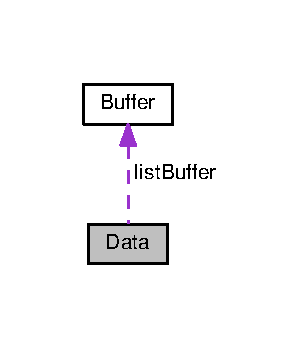
\includegraphics[width=145pt]{structData__coll__graph}
\end{center}
\end{figure}
\subsection*{Champs de données}
\begin{DoxyCompactItemize}
\item 
int {\bfseries trem}\hypertarget{structData_ab9d88ed9917ede02fe64d299cd7ee33e}{}\label{structData_ab9d88ed9917ede02fe64d299cd7ee33e}

\item 
float {\bfseries tremolo\+\_\+fc}\hypertarget{structData_a2f42f61ad1e519f4bd15d88c0b63a184}{}\label{structData_a2f42f61ad1e519f4bd15d88c0b63a184}

\item 
float {\bfseries tremolo\+\_\+alpha}\hypertarget{structData_a1e7d83c00e768ba6194921bf1a22766a}{}\label{structData_a1e7d83c00e768ba6194921bf1a22766a}

\item 
float {\bfseries wah}\hypertarget{structData_a53265f6c12c21b95ad5f0828d9b748aa}{}\label{structData_a53265f6c12c21b95ad5f0828d9b748aa}

\item 
int {\bfseries monte}\hypertarget{structData_af76c45e6e5edf309fa906d77b0fa4f41}{}\label{structData_af76c45e6e5edf309fa906d77b0fa4f41}

\item 
float {\bfseries wah\+\_\+fw}\hypertarget{structData_a5755f20c0c466ee6f8c2ef48234b83ba}{}\label{structData_a5755f20c0c466ee6f8c2ef48234b83ba}

\item 
int {\bfseries flange}\hypertarget{structData_ad088a0bb2b8fd8ef01c6e4a889004e35}{}\label{structData_ad088a0bb2b8fd8ef01c6e4a889004e35}

\item 
float {\bfseries flanger\+\_\+amp}\hypertarget{structData_a8e7e0d39e13b4ac2aaf93da0f8c9b859}{}\label{structData_a8e7e0d39e13b4ac2aaf93da0f8c9b859}

\item 
float {\bfseries flanger\+\_\+rate}\hypertarget{structData_a0b7b5cc28a48c53dd7cf79b39dd6d235}{}\label{structData_a0b7b5cc28a48c53dd7cf79b39dd6d235}

\item 
float {\bfseries flanger\+\_\+max\+\_\+time\+\_\+delay}\hypertarget{structData_ac2a7f5d469a9335a2b37fcbcef00650d}{}\label{structData_ac2a7f5d469a9335a2b37fcbcef00650d}

\item 
float {\bfseries chorus\+\_\+gain}\hypertarget{structData_a7ce19a1d32cc162a4599227142abac6b}{}\label{structData_a7ce19a1d32cc162a4599227142abac6b}

\item 
int {\bfseries choeur}\hypertarget{structData_abeda9313a40d5d26d05c8d5be57729ff}{}\label{structData_abeda9313a40d5d26d05c8d5be57729ff}

\item 
int {\bfseries chorus\+\_\+retard}\hypertarget{structData_ab57fd3fd528f25da771d6a78d87397dd}{}\label{structData_ab57fd3fd528f25da771d6a78d87397dd}

\item 
int {\bfseries chorus\+\_\+change}\hypertarget{structData_af2221f9b7ee9a4956c49e2f4082bf77c}{}\label{structData_af2221f9b7ee9a4956c49e2f4082bf77c}

\item 
float {\bfseries echo\+\_\+gain}\hypertarget{structData_a2c5e8f4c1996cff83c3c771a5e4c7fa4}{}\label{structData_a2c5e8f4c1996cff83c3c771a5e4c7fa4}

\item 
float {\bfseries echo\+\_\+retard}\hypertarget{structData_a3a723aa2c060f75a70ad64747788ee46}{}\label{structData_a3a723aa2c060f75a70ad64747788ee46}

\item 
float {\bfseries fuzz\+\_\+gain}\hypertarget{structData_a9851ce76f0c1af9d37b50234efc36194}{}\label{structData_a9851ce76f0c1af9d37b50234efc36194}

\item 
float {\bfseries fuzz\+\_\+mix}\hypertarget{structData_a2b998d1c5dda077fbee1bf14c6d805c7}{}\label{structData_a2b998d1c5dda077fbee1bf14c6d805c7}

\item 
int {\bfseries overdrive\+\_\+drive}\hypertarget{structData_a046a8d98bbef53a2a35013659bbe7a89}{}\label{structData_a046a8d98bbef53a2a35013659bbe7a89}

\item 
float {\bfseries vibrato\+\_\+modfreq}\hypertarget{structData_a9d88709c1bfb8cdb57f3022ac3795c7c}{}\label{structData_a9d88709c1bfb8cdb57f3022ac3795c7c}

\item 
float {\bfseries vibrato\+\_\+width}\hypertarget{structData_aa457c0bec259ad4f72a749c0d7cba67c}{}\label{structData_aa457c0bec259ad4f72a749c0d7cba67c}

\item 
int {\bfseries vibre}\hypertarget{structData_ab76b1197ccfe12ef51640e6c42eb2b9a}{}\label{structData_ab76b1197ccfe12ef51640e6c42eb2b9a}

\item 
float {\bfseries shelving\+\_\+gain}\hypertarget{structData_a36a0702688d5a835c7189846131a6487}{}\label{structData_a36a0702688d5a835c7189846131a6487}

\item 
float {\bfseries shelving\+\_\+fc}\hypertarget{structData_acc41c5321d720af7ef090304d57bebbe}{}\label{structData_acc41c5321d720af7ef090304d57bebbe}

\item 
float {\bfseries shelving\+\_\+Q}\hypertarget{structData_a94dc3fd1f3e36f82829b924f50635261}{}\label{structData_a94dc3fd1f3e36f82829b924f50635261}

\item 
EQ {\bfseries shelving\+\_\+type}\hypertarget{structData_afa24b396e1bab1c62d9f907f612d84e5}{}\label{structData_afa24b396e1bab1c62d9f907f612d84e5}

\item 
\hyperlink{structBuffer}{Buffer} $\ast$ {\bfseries list\+Buffer}\hypertarget{structData_ad8144307f2fe566d717719a07ae3fd36}{}\label{structData_ad8144307f2fe566d717719a07ae3fd36}

\item 
E\+T\+AT {\bfseries effets} \mbox{[}N\+B\+\_\+\+E\+F\+F\+E\+TS\mbox{]}\hypertarget{structData_aec895ebeebd83409b566dbab730e38d2}{}\label{structData_aec895ebeebd83409b566dbab730e38d2}

\end{DoxyCompactItemize}


\subsection{Description détaillée}
Paramètres des effets. 

\subsection{Documentation des champs}
\index{Data@{Data}!choeur@{choeur}}
\index{choeur@{choeur}!Data@{Data}}
\subsubsection[{\texorpdfstring{choeur}{choeur}}]{\setlength{\rightskip}{0pt plus 5cm}int Data\+::choeur}\hypertarget{structData_abeda9313a40d5d26d05c8d5be57729ff}{}\label{structData_abeda9313a40d5d26d05c8d5be57729ff}
\index{Data@{Data}!chorus\+\_\+change@{chorus\+\_\+change}}
\index{chorus\+\_\+change@{chorus\+\_\+change}!Data@{Data}}
\subsubsection[{\texorpdfstring{chorus\+\_\+change}{chorus_change}}]{\setlength{\rightskip}{0pt plus 5cm}int Data\+::chorus\+\_\+change}\hypertarget{structData_af2221f9b7ee9a4956c49e2f4082bf77c}{}\label{structData_af2221f9b7ee9a4956c49e2f4082bf77c}
\index{Data@{Data}!chorus\+\_\+gain@{chorus\+\_\+gain}}
\index{chorus\+\_\+gain@{chorus\+\_\+gain}!Data@{Data}}
\subsubsection[{\texorpdfstring{chorus\+\_\+gain}{chorus_gain}}]{\setlength{\rightskip}{0pt plus 5cm}float Data\+::chorus\+\_\+gain}\hypertarget{structData_a7ce19a1d32cc162a4599227142abac6b}{}\label{structData_a7ce19a1d32cc162a4599227142abac6b}
\index{Data@{Data}!chorus\+\_\+retard@{chorus\+\_\+retard}}
\index{chorus\+\_\+retard@{chorus\+\_\+retard}!Data@{Data}}
\subsubsection[{\texorpdfstring{chorus\+\_\+retard}{chorus_retard}}]{\setlength{\rightskip}{0pt plus 5cm}int Data\+::chorus\+\_\+retard}\hypertarget{structData_ab57fd3fd528f25da771d6a78d87397dd}{}\label{structData_ab57fd3fd528f25da771d6a78d87397dd}
\index{Data@{Data}!echo\+\_\+gain@{echo\+\_\+gain}}
\index{echo\+\_\+gain@{echo\+\_\+gain}!Data@{Data}}
\subsubsection[{\texorpdfstring{echo\+\_\+gain}{echo_gain}}]{\setlength{\rightskip}{0pt plus 5cm}float Data\+::echo\+\_\+gain}\hypertarget{structData_a2c5e8f4c1996cff83c3c771a5e4c7fa4}{}\label{structData_a2c5e8f4c1996cff83c3c771a5e4c7fa4}
\index{Data@{Data}!echo\+\_\+retard@{echo\+\_\+retard}}
\index{echo\+\_\+retard@{echo\+\_\+retard}!Data@{Data}}
\subsubsection[{\texorpdfstring{echo\+\_\+retard}{echo_retard}}]{\setlength{\rightskip}{0pt plus 5cm}float Data\+::echo\+\_\+retard}\hypertarget{structData_a3a723aa2c060f75a70ad64747788ee46}{}\label{structData_a3a723aa2c060f75a70ad64747788ee46}
\index{Data@{Data}!effets@{effets}}
\index{effets@{effets}!Data@{Data}}
\subsubsection[{\texorpdfstring{effets}{effets}}]{\setlength{\rightskip}{0pt plus 5cm}E\+T\+AT Data\+::effets\mbox{[}N\+B\+\_\+\+E\+F\+F\+E\+TS\mbox{]}}\hypertarget{structData_aec895ebeebd83409b566dbab730e38d2}{}\label{structData_aec895ebeebd83409b566dbab730e38d2}
\index{Data@{Data}!flange@{flange}}
\index{flange@{flange}!Data@{Data}}
\subsubsection[{\texorpdfstring{flange}{flange}}]{\setlength{\rightskip}{0pt plus 5cm}int Data\+::flange}\hypertarget{structData_ad088a0bb2b8fd8ef01c6e4a889004e35}{}\label{structData_ad088a0bb2b8fd8ef01c6e4a889004e35}
\index{Data@{Data}!flanger\+\_\+amp@{flanger\+\_\+amp}}
\index{flanger\+\_\+amp@{flanger\+\_\+amp}!Data@{Data}}
\subsubsection[{\texorpdfstring{flanger\+\_\+amp}{flanger_amp}}]{\setlength{\rightskip}{0pt plus 5cm}float Data\+::flanger\+\_\+amp}\hypertarget{structData_a8e7e0d39e13b4ac2aaf93da0f8c9b859}{}\label{structData_a8e7e0d39e13b4ac2aaf93da0f8c9b859}
\index{Data@{Data}!flanger\+\_\+max\+\_\+time\+\_\+delay@{flanger\+\_\+max\+\_\+time\+\_\+delay}}
\index{flanger\+\_\+max\+\_\+time\+\_\+delay@{flanger\+\_\+max\+\_\+time\+\_\+delay}!Data@{Data}}
\subsubsection[{\texorpdfstring{flanger\+\_\+max\+\_\+time\+\_\+delay}{flanger_max_time_delay}}]{\setlength{\rightskip}{0pt plus 5cm}float Data\+::flanger\+\_\+max\+\_\+time\+\_\+delay}\hypertarget{structData_ac2a7f5d469a9335a2b37fcbcef00650d}{}\label{structData_ac2a7f5d469a9335a2b37fcbcef00650d}
\index{Data@{Data}!flanger\+\_\+rate@{flanger\+\_\+rate}}
\index{flanger\+\_\+rate@{flanger\+\_\+rate}!Data@{Data}}
\subsubsection[{\texorpdfstring{flanger\+\_\+rate}{flanger_rate}}]{\setlength{\rightskip}{0pt plus 5cm}float Data\+::flanger\+\_\+rate}\hypertarget{structData_a0b7b5cc28a48c53dd7cf79b39dd6d235}{}\label{structData_a0b7b5cc28a48c53dd7cf79b39dd6d235}
\index{Data@{Data}!fuzz\+\_\+gain@{fuzz\+\_\+gain}}
\index{fuzz\+\_\+gain@{fuzz\+\_\+gain}!Data@{Data}}
\subsubsection[{\texorpdfstring{fuzz\+\_\+gain}{fuzz_gain}}]{\setlength{\rightskip}{0pt plus 5cm}float Data\+::fuzz\+\_\+gain}\hypertarget{structData_a9851ce76f0c1af9d37b50234efc36194}{}\label{structData_a9851ce76f0c1af9d37b50234efc36194}
\index{Data@{Data}!fuzz\+\_\+mix@{fuzz\+\_\+mix}}
\index{fuzz\+\_\+mix@{fuzz\+\_\+mix}!Data@{Data}}
\subsubsection[{\texorpdfstring{fuzz\+\_\+mix}{fuzz_mix}}]{\setlength{\rightskip}{0pt plus 5cm}float Data\+::fuzz\+\_\+mix}\hypertarget{structData_a2b998d1c5dda077fbee1bf14c6d805c7}{}\label{structData_a2b998d1c5dda077fbee1bf14c6d805c7}
\index{Data@{Data}!list\+Buffer@{list\+Buffer}}
\index{list\+Buffer@{list\+Buffer}!Data@{Data}}
\subsubsection[{\texorpdfstring{list\+Buffer}{listBuffer}}]{\setlength{\rightskip}{0pt plus 5cm}{\bf Buffer}$\ast$ Data\+::list\+Buffer}\hypertarget{structData_ad8144307f2fe566d717719a07ae3fd36}{}\label{structData_ad8144307f2fe566d717719a07ae3fd36}
\index{Data@{Data}!monte@{monte}}
\index{monte@{monte}!Data@{Data}}
\subsubsection[{\texorpdfstring{monte}{monte}}]{\setlength{\rightskip}{0pt plus 5cm}int Data\+::monte}\hypertarget{structData_af76c45e6e5edf309fa906d77b0fa4f41}{}\label{structData_af76c45e6e5edf309fa906d77b0fa4f41}
\index{Data@{Data}!overdrive\+\_\+drive@{overdrive\+\_\+drive}}
\index{overdrive\+\_\+drive@{overdrive\+\_\+drive}!Data@{Data}}
\subsubsection[{\texorpdfstring{overdrive\+\_\+drive}{overdrive_drive}}]{\setlength{\rightskip}{0pt plus 5cm}int Data\+::overdrive\+\_\+drive}\hypertarget{structData_a046a8d98bbef53a2a35013659bbe7a89}{}\label{structData_a046a8d98bbef53a2a35013659bbe7a89}
\index{Data@{Data}!shelving\+\_\+fc@{shelving\+\_\+fc}}
\index{shelving\+\_\+fc@{shelving\+\_\+fc}!Data@{Data}}
\subsubsection[{\texorpdfstring{shelving\+\_\+fc}{shelving_fc}}]{\setlength{\rightskip}{0pt plus 5cm}float Data\+::shelving\+\_\+fc}\hypertarget{structData_acc41c5321d720af7ef090304d57bebbe}{}\label{structData_acc41c5321d720af7ef090304d57bebbe}
\index{Data@{Data}!shelving\+\_\+gain@{shelving\+\_\+gain}}
\index{shelving\+\_\+gain@{shelving\+\_\+gain}!Data@{Data}}
\subsubsection[{\texorpdfstring{shelving\+\_\+gain}{shelving_gain}}]{\setlength{\rightskip}{0pt plus 5cm}float Data\+::shelving\+\_\+gain}\hypertarget{structData_a36a0702688d5a835c7189846131a6487}{}\label{structData_a36a0702688d5a835c7189846131a6487}
\index{Data@{Data}!shelving\+\_\+Q@{shelving\+\_\+Q}}
\index{shelving\+\_\+Q@{shelving\+\_\+Q}!Data@{Data}}
\subsubsection[{\texorpdfstring{shelving\+\_\+Q}{shelving_Q}}]{\setlength{\rightskip}{0pt plus 5cm}float Data\+::shelving\+\_\+Q}\hypertarget{structData_a94dc3fd1f3e36f82829b924f50635261}{}\label{structData_a94dc3fd1f3e36f82829b924f50635261}
\index{Data@{Data}!shelving\+\_\+type@{shelving\+\_\+type}}
\index{shelving\+\_\+type@{shelving\+\_\+type}!Data@{Data}}
\subsubsection[{\texorpdfstring{shelving\+\_\+type}{shelving_type}}]{\setlength{\rightskip}{0pt plus 5cm}EQ Data\+::shelving\+\_\+type}\hypertarget{structData_afa24b396e1bab1c62d9f907f612d84e5}{}\label{structData_afa24b396e1bab1c62d9f907f612d84e5}
\index{Data@{Data}!trem@{trem}}
\index{trem@{trem}!Data@{Data}}
\subsubsection[{\texorpdfstring{trem}{trem}}]{\setlength{\rightskip}{0pt plus 5cm}int Data\+::trem}\hypertarget{structData_ab9d88ed9917ede02fe64d299cd7ee33e}{}\label{structData_ab9d88ed9917ede02fe64d299cd7ee33e}
\index{Data@{Data}!tremolo\+\_\+alpha@{tremolo\+\_\+alpha}}
\index{tremolo\+\_\+alpha@{tremolo\+\_\+alpha}!Data@{Data}}
\subsubsection[{\texorpdfstring{tremolo\+\_\+alpha}{tremolo_alpha}}]{\setlength{\rightskip}{0pt plus 5cm}float Data\+::tremolo\+\_\+alpha}\hypertarget{structData_a1e7d83c00e768ba6194921bf1a22766a}{}\label{structData_a1e7d83c00e768ba6194921bf1a22766a}
\index{Data@{Data}!tremolo\+\_\+fc@{tremolo\+\_\+fc}}
\index{tremolo\+\_\+fc@{tremolo\+\_\+fc}!Data@{Data}}
\subsubsection[{\texorpdfstring{tremolo\+\_\+fc}{tremolo_fc}}]{\setlength{\rightskip}{0pt plus 5cm}float Data\+::tremolo\+\_\+fc}\hypertarget{structData_a2f42f61ad1e519f4bd15d88c0b63a184}{}\label{structData_a2f42f61ad1e519f4bd15d88c0b63a184}
\index{Data@{Data}!vibrato\+\_\+modfreq@{vibrato\+\_\+modfreq}}
\index{vibrato\+\_\+modfreq@{vibrato\+\_\+modfreq}!Data@{Data}}
\subsubsection[{\texorpdfstring{vibrato\+\_\+modfreq}{vibrato_modfreq}}]{\setlength{\rightskip}{0pt plus 5cm}float Data\+::vibrato\+\_\+modfreq}\hypertarget{structData_a9d88709c1bfb8cdb57f3022ac3795c7c}{}\label{structData_a9d88709c1bfb8cdb57f3022ac3795c7c}
\index{Data@{Data}!vibrato\+\_\+width@{vibrato\+\_\+width}}
\index{vibrato\+\_\+width@{vibrato\+\_\+width}!Data@{Data}}
\subsubsection[{\texorpdfstring{vibrato\+\_\+width}{vibrato_width}}]{\setlength{\rightskip}{0pt plus 5cm}float Data\+::vibrato\+\_\+width}\hypertarget{structData_aa457c0bec259ad4f72a749c0d7cba67c}{}\label{structData_aa457c0bec259ad4f72a749c0d7cba67c}
\index{Data@{Data}!vibre@{vibre}}
\index{vibre@{vibre}!Data@{Data}}
\subsubsection[{\texorpdfstring{vibre}{vibre}}]{\setlength{\rightskip}{0pt plus 5cm}int Data\+::vibre}\hypertarget{structData_ab76b1197ccfe12ef51640e6c42eb2b9a}{}\label{structData_ab76b1197ccfe12ef51640e6c42eb2b9a}
\index{Data@{Data}!wah@{wah}}
\index{wah@{wah}!Data@{Data}}
\subsubsection[{\texorpdfstring{wah}{wah}}]{\setlength{\rightskip}{0pt plus 5cm}float Data\+::wah}\hypertarget{structData_a53265f6c12c21b95ad5f0828d9b748aa}{}\label{structData_a53265f6c12c21b95ad5f0828d9b748aa}
\index{Data@{Data}!wah\+\_\+fw@{wah\+\_\+fw}}
\index{wah\+\_\+fw@{wah\+\_\+fw}!Data@{Data}}
\subsubsection[{\texorpdfstring{wah\+\_\+fw}{wah_fw}}]{\setlength{\rightskip}{0pt plus 5cm}float Data\+::wah\+\_\+fw}\hypertarget{structData_a5755f20c0c466ee6f8c2ef48234b83ba}{}\label{structData_a5755f20c0c466ee6f8c2ef48234b83ba}


La documentation de cette structure a été générée à partir du fichier suivant \+:\begin{DoxyCompactItemize}
\item 
header/prototypes.\+h\end{DoxyCompactItemize}

\hypertarget{structPedale}{}\section{Référence de la structure Pedale}
\label{structPedale}\index{Pedale@{Pedale}}
\subsection*{Champs de données}
\begin{DoxyCompactItemize}
\item 
char {\bfseries nom} \mbox{[}20\mbox{]}\hypertarget{structPedale_aadad624255828e83c18a11df31c8f559}{}\label{structPedale_aadad624255828e83c18a11df31c8f559}

\item 
S\+D\+L\+\_\+\+Rect {\bfseries position}\hypertarget{structPedale_ac06cf6a292dc0e70e28b394fa481aef2}{}\label{structPedale_ac06cf6a292dc0e70e28b394fa481aef2}

\item 
S\+D\+L\+\_\+\+Surface $\ast$ {\bfseries texte}\hypertarget{structPedale_a5b66158197948c551bbf808da9f95726}{}\label{structPedale_a5b66158197948c551bbf808da9f95726}

\end{DoxyCompactItemize}


La documentation de cette structure a été générée à partir du fichier suivant \+:\begin{DoxyCompactItemize}
\item 
affichage.\+h\end{DoxyCompactItemize}

\chapter{Documentation des fichiers}
\input{affichage_8c}
\hypertarget{audio_8c}{}\section{Référence du fichier src/audio.c}
\label{audio_8c}\index{src/audio.\+c@{src/audio.\+c}}


Fichier gérant l\textquotesingle{}implémentation des effets.  


{\ttfamily \#include $<$stdlib.\+h$>$}\\*
{\ttfamily \#include $<$stdio.\+h$>$}\\*
{\ttfamily \#include $<$math.\+h$>$}\\*
{\ttfamily \#include $<$time.\+h$>$}\\*
{\ttfamily \#include \char`\"{}../header/prototypes.\+h\char`\"{}}\\*
{\ttfamily \#include \char`\"{}../header/audio.\+h\char`\"{}}\\*
Graphe des dépendances par inclusion de audio.\+c\+:\nopagebreak
\begin{figure}[H]
\begin{center}
\leavevmode
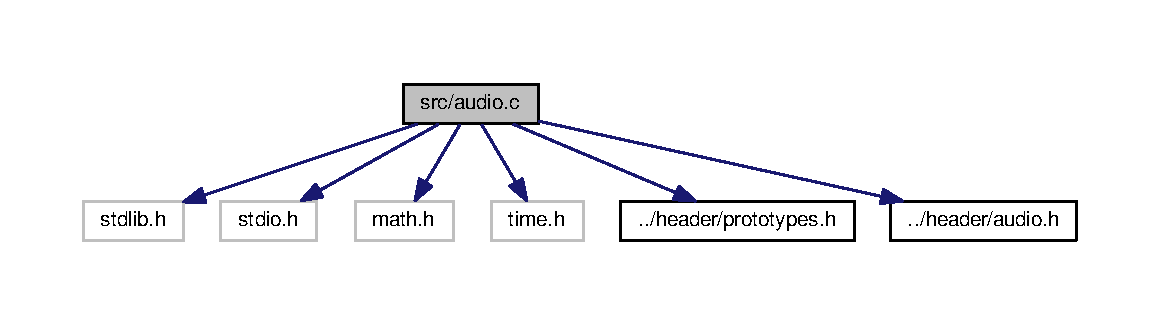
\includegraphics[width=350pt]{audio_8c__incl}
\end{center}
\end{figure}
\subsection*{Fonctions}
\begin{DoxyCompactItemize}
\item 
void \hyperlink{audio_8c_a3e7867b1e230dc6f63c5d6572379fee2}{copie} (float $\ast$src, float $\ast$dest)
\begin{DoxyCompactList}\small\item\em Copie un tableau dans un autre. \end{DoxyCompactList}\item 
void \hyperlink{audio_8c_abc8a4cb48273e1a25a5036c688e10cc1}{fuzz} (float $\ast$in, float $\ast$out, float gain, float mix)
\begin{DoxyCompactList}\small\item\em Applique un effet fuzz au son. \end{DoxyCompactList}\item 
void \hyperlink{audio_8c_acaa7183c60d77c306a447aaa4aa72201}{overdrive} (float $\ast$in, float $\ast$out, int drive)
\begin{DoxyCompactList}\small\item\em Applique l\textquotesingle{}effet overdrive au son. \end{DoxyCompactList}\item 
void \hyperlink{audio_8c_a9b52b9ea406a57d166295da272e3d8b9}{wahwah} (float $\ast$in, float $\ast$out, int fw, float $\ast$wah, int $\ast$monte)
\begin{DoxyCompactList}\small\item\em Applique un effet wah-\/wah automatique au signal. \end{DoxyCompactList}\item 
void \hyperlink{audio_8c_a5c20ec4b8b7d35d17d75978ea0849ce5}{tremolo} (float $\ast$in, float $\ast$out, float alpha, float fc, int $\ast$trem)
\begin{DoxyCompactList}\small\item\em Applique un effet tremolo au signal. \end{DoxyCompactList}\item 
void \hyperlink{audio_8c_aa5af6c6e5968aca623175887be170409}{echo} (float $\ast$in, float $\ast$out, float gain, float retard, \hyperlink{structBuffer}{Buffer} $\ast$list\+Buffer)
\begin{DoxyCompactList}\small\item\em Applique un effet echo au signal. \end{DoxyCompactList}\item 
void \hyperlink{audio_8c_a1e8fefad8f9c1a3ac0429ce6bdfa5772}{flanger} (float $\ast$in, float $\ast$out, float amp, \hyperlink{structBuffer}{Buffer} $\ast$list\+Buffer, float max\+\_\+time\+\_\+delay, float rate, int $\ast$flange)
\begin{DoxyCompactList}\small\item\em Applique l\textquotesingle{}effet flanger au signal. \end{DoxyCompactList}\item 
void \hyperlink{audio_8c_a9a05bafc2202fcd24b204620624ffd82}{chorus} (float $\ast$in, float $\ast$out, float gain, \hyperlink{structBuffer}{Buffer} $\ast$list\+Buffer, int $\ast$choeur, int $\ast$retard, int change)
\begin{DoxyCompactList}\small\item\em Applique l\textquotesingle{}effet chorus au signal. \end{DoxyCompactList}\item 
void \hyperlink{audio_8c_a731dfba06c905935b44269f7a4bbfbed}{filter} (float $\ast$b, float $\ast$a, int nb, int na, float $\ast$in, float $\ast$out)
\begin{DoxyCompactList}\small\item\em Effectue un filtrage linéaire selon une fonction de transfert rationelle. \end{DoxyCompactList}\item 
void \hyperlink{audio_8c_a04331f5e0a564fb1723cc3def0990de0}{shelving} (float $\ast$in, float $\ast$out, float gain, float fc, EQ type)
\begin{DoxyCompactList}\small\item\em Applique un filtre shelving au signal. \end{DoxyCompactList}\item 
void \hyperlink{audio_8c_a04cd0027e1c74860543a0a0375e85c9a}{vibrato} (float $\ast$in, float $\ast$out, float modfreq, float width, int $\ast$vibre)
\begin{DoxyCompactList}\small\item\em Applique un effet vibrato au signal. \end{DoxyCompactList}\end{DoxyCompactItemize}


\subsection{Description détaillée}
Fichier gérant l\textquotesingle{}implémentation des effets. 



\subsection{Documentation des fonctions}
\index{audio.\+c@{audio.\+c}!chorus@{chorus}}
\index{chorus@{chorus}!audio.\+c@{audio.\+c}}
\subsubsection[{\texorpdfstring{chorus(float $\ast$in, float $\ast$out, float gain, Buffer $\ast$list\+Buffer, int $\ast$choeur, int $\ast$retard, int change)}{chorus(float *in, float *out, float gain, Buffer *listBuffer, int *choeur, int *retard, int change)}}]{\setlength{\rightskip}{0pt plus 5cm}void chorus (
\begin{DoxyParamCaption}
\item[{float $\ast$}]{in, }
\item[{float $\ast$}]{out, }
\item[{float}]{gain, }
\item[{{\bf Buffer} $\ast$}]{list\+Buffer, }
\item[{int $\ast$}]{choeur, }
\item[{int $\ast$}]{retard, }
\item[{int}]{change}
\end{DoxyParamCaption}
)}\hypertarget{audio_8c_a9a05bafc2202fcd24b204620624ffd82}{}\label{audio_8c_a9a05bafc2202fcd24b204620624ffd82}


Applique l\textquotesingle{}effet chorus au signal. 


\begin{DoxyParams}{Paramètres}
{\em in} & Le buffer d\textquotesingle{}entrée \\
\hline
{\em out} & Le buffer de sortie \\
\hline
{\em gain} & Niveau de gain \\
\hline
{\em list\+Buffer} & La liste des buffer en mémoire \\
\hline
{\em choeur} & Compteur du nombre d\textquotesingle{}échantillon traités \\
\hline
{\em retard} & Le retard de l\textquotesingle{}effet (calculé dans la fonction) \\
\hline
{\em change} & Indicateur du nombre d\textquotesingle{}échantillons à traiter avant de changer le retard \\
\hline
\end{DoxyParams}
\index{audio.\+c@{audio.\+c}!copie@{copie}}
\index{copie@{copie}!audio.\+c@{audio.\+c}}
\subsubsection[{\texorpdfstring{copie(float $\ast$src, float $\ast$dest)}{copie(float *src, float *dest)}}]{\setlength{\rightskip}{0pt plus 5cm}void copie (
\begin{DoxyParamCaption}
\item[{float $\ast$}]{src, }
\item[{float $\ast$}]{dest}
\end{DoxyParamCaption}
)}\hypertarget{audio_8c_a3e7867b1e230dc6f63c5d6572379fee2}{}\label{audio_8c_a3e7867b1e230dc6f63c5d6572379fee2}


Copie un tableau dans un autre. 


\begin{DoxyParams}{Paramètres}
{\em src} & Tableau source \\
\hline
{\em dest} & Tableau de destination \\
\hline
\end{DoxyParams}
\index{audio.\+c@{audio.\+c}!echo@{echo}}
\index{echo@{echo}!audio.\+c@{audio.\+c}}
\subsubsection[{\texorpdfstring{echo(float $\ast$in, float $\ast$out, float gain, float retard, Buffer $\ast$list\+Buffer)}{echo(float *in, float *out, float gain, float retard, Buffer *listBuffer)}}]{\setlength{\rightskip}{0pt plus 5cm}void echo (
\begin{DoxyParamCaption}
\item[{float $\ast$}]{in, }
\item[{float $\ast$}]{out, }
\item[{float}]{gain, }
\item[{float}]{retard, }
\item[{{\bf Buffer} $\ast$}]{list\+Buffer}
\end{DoxyParamCaption}
)}\hypertarget{audio_8c_aa5af6c6e5968aca623175887be170409}{}\label{audio_8c_aa5af6c6e5968aca623175887be170409}


Applique un effet echo au signal. 


\begin{DoxyParams}{Paramètres}
{\em in} & Le buffer d\textquotesingle{}entrée \\
\hline
{\em out} & le buffer de sortie \\
\hline
{\em gain} & Niveau de gain \\
\hline
{\em retard} & Le retard en ms de l\textquotesingle{}echo \\
\hline
{\em list\+Buffer} & La liste des buffer en mémoire \\
\hline
\end{DoxyParams}
\index{audio.\+c@{audio.\+c}!filter@{filter}}
\index{filter@{filter}!audio.\+c@{audio.\+c}}
\subsubsection[{\texorpdfstring{filter(float $\ast$b, float $\ast$a, int nb, int na, float $\ast$in, float $\ast$out)}{filter(float *b, float *a, int nb, int na, float *in, float *out)}}]{\setlength{\rightskip}{0pt plus 5cm}void filter (
\begin{DoxyParamCaption}
\item[{float $\ast$}]{b, }
\item[{float $\ast$}]{a, }
\item[{int}]{nb, }
\item[{int}]{na, }
\item[{float $\ast$}]{in, }
\item[{float $\ast$}]{out}
\end{DoxyParamCaption}
)}\hypertarget{audio_8c_a731dfba06c905935b44269f7a4bbfbed}{}\label{audio_8c_a731dfba06c905935b44269f7a4bbfbed}


Effectue un filtrage linéaire selon une fonction de transfert rationelle. 

$ a[0]y[n] = b[0]x[n] + b[1]x[n-1] + ... + b[nb-1]x[n-(nb-1)] - a[1]x[n-1] - ... - a[na-1]x[n-(na-1)] $ 
\begin{DoxyParams}{Paramètres}
{\em b} & Coefficient du numérateur \\
\hline
{\em a} & Coefficient du dénominateur \\
\hline
{\em nb} & Taille de b \\
\hline
{\em na} & Taille de a \\
\hline
{\em in} & Le buffer d\textquotesingle{}entrée \\
\hline
{\em out} & Le buffer de sortie \\
\hline
\end{DoxyParams}
\index{audio.\+c@{audio.\+c}!flanger@{flanger}}
\index{flanger@{flanger}!audio.\+c@{audio.\+c}}
\subsubsection[{\texorpdfstring{flanger(float $\ast$in, float $\ast$out, float amp, Buffer $\ast$list\+Buffer, float max\+\_\+time\+\_\+delay, float rate, int $\ast$flange)}{flanger(float *in, float *out, float amp, Buffer *listBuffer, float max_time_delay, float rate, int *flange)}}]{\setlength{\rightskip}{0pt plus 5cm}void flanger (
\begin{DoxyParamCaption}
\item[{float $\ast$}]{in, }
\item[{float $\ast$}]{out, }
\item[{float}]{amp, }
\item[{{\bf Buffer} $\ast$}]{list\+Buffer, }
\item[{float}]{max\+\_\+time\+\_\+delay, }
\item[{float}]{rate, }
\item[{int $\ast$}]{flange}
\end{DoxyParamCaption}
)}\hypertarget{audio_8c_a1e8fefad8f9c1a3ac0429ce6bdfa5772}{}\label{audio_8c_a1e8fefad8f9c1a3ac0429ce6bdfa5772}


Applique l\textquotesingle{}effet flanger au signal. 


\begin{DoxyParams}{Paramètres}
{\em in} & Le buffer d\textquotesingle{}entrée \\
\hline
{\em out} & Le buffer de sortie \\
\hline
{\em amp} & Niveau d\textquotesingle{}amplification \\
\hline
{\em list\+Buffer} & La liste des buffer en mémoire \\
\hline
{\em max\+\_\+time\+\_\+delay} & Le delay du retard en secondes compris entre 3ms et 15ms \\
\hline
{\em rate} & Pourcentage de flange en Hz \\
\hline
{\em flange} & Pour éviter de revenir au début de la sinusoide à chaque nouveau buffer \\
\hline
\end{DoxyParams}
\index{audio.\+c@{audio.\+c}!fuzz@{fuzz}}
\index{fuzz@{fuzz}!audio.\+c@{audio.\+c}}
\subsubsection[{\texorpdfstring{fuzz(float $\ast$in, float $\ast$out, float gain, float mix)}{fuzz(float *in, float *out, float gain, float mix)}}]{\setlength{\rightskip}{0pt plus 5cm}void fuzz (
\begin{DoxyParamCaption}
\item[{float $\ast$}]{in, }
\item[{float $\ast$}]{out, }
\item[{float}]{gain, }
\item[{float}]{mix}
\end{DoxyParamCaption}
)}\hypertarget{audio_8c_abc8a4cb48273e1a25a5036c688e10cc1}{}\label{audio_8c_abc8a4cb48273e1a25a5036c688e10cc1}


Applique un effet fuzz au son. 


\begin{DoxyParams}{Paramètres}
{\em in} & \hyperlink{structBuffer}{Buffer} d\textquotesingle{}entree du son \\
\hline
{\em out} & buffer de sortie du son \\
\hline
{\em gain} & Montant de distortion \\
\hline
{\em mix} & Mix du signal distordu et original \\
\hline
\end{DoxyParams}
\begin{DoxyWarning}{Avertissement}
mix doit être comprix entre 0 et 1 
\end{DoxyWarning}
\index{audio.\+c@{audio.\+c}!overdrive@{overdrive}}
\index{overdrive@{overdrive}!audio.\+c@{audio.\+c}}
\subsubsection[{\texorpdfstring{overdrive(float $\ast$in, float $\ast$out, int drive)}{overdrive(float *in, float *out, int drive)}}]{\setlength{\rightskip}{0pt plus 5cm}void overdrive (
\begin{DoxyParamCaption}
\item[{float $\ast$}]{in, }
\item[{float $\ast$}]{out, }
\item[{int}]{drive}
\end{DoxyParamCaption}
)}\hypertarget{audio_8c_acaa7183c60d77c306a447aaa4aa72201}{}\label{audio_8c_acaa7183c60d77c306a447aaa4aa72201}


Applique l\textquotesingle{}effet overdrive au son. 

On appelle la fonction récursivement pour augmenter l\textquotesingle{}effet 
\begin{DoxyParams}{Paramètres}
{\em in} & le buffer d\textquotesingle{}entrée \\
\hline
{\em out} & le buffer de sortie \\
\hline
{\em drive} & Nombre d\textquotesingle{}appel récursif \\
\hline
\end{DoxyParams}
\index{audio.\+c@{audio.\+c}!shelving@{shelving}}
\index{shelving@{shelving}!audio.\+c@{audio.\+c}}
\subsubsection[{\texorpdfstring{shelving(float $\ast$in, float $\ast$out, float gain, float fc, E\+Q type)}{shelving(float *in, float *out, float gain, float fc, EQ type)}}]{\setlength{\rightskip}{0pt plus 5cm}void shelving (
\begin{DoxyParamCaption}
\item[{float $\ast$}]{in, }
\item[{float $\ast$}]{out, }
\item[{float}]{gain, }
\item[{float}]{fc, }
\item[{EQ}]{type}
\end{DoxyParamCaption}
)}\hypertarget{audio_8c_a04331f5e0a564fb1723cc3def0990de0}{}\label{audio_8c_a04331f5e0a564fb1723cc3def0990de0}


Applique un filtre shelving au signal. 


\begin{DoxyParams}{Paramètres}
{\em in} & Le buffer d\textquotesingle{}entrée \\
\hline
{\em out} & Le buffer de sortie \\
\hline
{\em gain} & Niveau de gain. Un gain positif provoque un boost des fréquences et un gain négatif provoque un cut. \\
\hline
{\em fc} & La fréquence centrale \\
\hline
{\em type} & Le type d\textquotesingle{}égalisation. (B\+A\+SS, T\+R\+E\+B\+LE ou A\+LL) \\
\hline
\end{DoxyParams}
\index{audio.\+c@{audio.\+c}!tremolo@{tremolo}}
\index{tremolo@{tremolo}!audio.\+c@{audio.\+c}}
\subsubsection[{\texorpdfstring{tremolo(float $\ast$in, float $\ast$out, float alpha, float fc, int $\ast$trem)}{tremolo(float *in, float *out, float alpha, float fc, int *trem)}}]{\setlength{\rightskip}{0pt plus 5cm}void tremolo (
\begin{DoxyParamCaption}
\item[{float $\ast$}]{in, }
\item[{float $\ast$}]{out, }
\item[{float}]{alpha, }
\item[{float}]{fc, }
\item[{int $\ast$}]{trem}
\end{DoxyParamCaption}
)}\hypertarget{audio_8c_a5c20ec4b8b7d35d17d75978ea0849ce5}{}\label{audio_8c_a5c20ec4b8b7d35d17d75978ea0849ce5}


Applique un effet tremolo au signal. 


\begin{DoxyParams}{Paramètres}
{\em in} & Le buffer d\textquotesingle{}entrée \\
\hline
{\em out} & Le buffer de sortie \\
\hline
{\em alpha} & Mixage signal d\textquotesingle{}entrée et modulation. Il est compris entre 0 et 1 sachant que 0 eteint la modulation et 1 donne le maximum de la modulation \\
\hline
{\em fc} & La fréquence de modulation \\
\hline
{\em trem} & Pour appliquer le tremolo en continu et ne pas recommencer à 0 sur chaque échantillon \\
\hline
\end{DoxyParams}
\index{audio.\+c@{audio.\+c}!vibrato@{vibrato}}
\index{vibrato@{vibrato}!audio.\+c@{audio.\+c}}
\subsubsection[{\texorpdfstring{vibrato(float $\ast$in, float $\ast$out, float modfreq, float width, int $\ast$vibre)}{vibrato(float *in, float *out, float modfreq, float width, int *vibre)}}]{\setlength{\rightskip}{0pt plus 5cm}void vibrato (
\begin{DoxyParamCaption}
\item[{float $\ast$}]{in, }
\item[{float $\ast$}]{out, }
\item[{float}]{modfreq, }
\item[{float}]{width, }
\item[{int $\ast$}]{vibre}
\end{DoxyParamCaption}
)}\hypertarget{audio_8c_a04cd0027e1c74860543a0a0375e85c9a}{}\label{audio_8c_a04cd0027e1c74860543a0a0375e85c9a}


Applique un effet vibrato au signal. 


\begin{DoxyParams}{Paramètres}
{\em in} & Le buffer d\textquotesingle{}entrée \\
\hline
{\em out} & Le buffer de sortie \\
\hline
{\em modfreq} & La fréquence de modulation en Hz \\
\hline
{\em width} & La largeur du retard en ms. \\
\hline
{\em vibre} & Compteur pour éviter de revenir au début de la sinusoide à chaque buffer \\
\hline
\end{DoxyParams}
\index{audio.\+c@{audio.\+c}!wahwah@{wahwah}}
\index{wahwah@{wahwah}!audio.\+c@{audio.\+c}}
\subsubsection[{\texorpdfstring{wahwah(float $\ast$in, float $\ast$out, int fw, float $\ast$wah, int $\ast$monte)}{wahwah(float *in, float *out, int fw, float *wah, int *monte)}}]{\setlength{\rightskip}{0pt plus 5cm}void wahwah (
\begin{DoxyParamCaption}
\item[{float $\ast$}]{in, }
\item[{float $\ast$}]{out, }
\item[{int}]{fw, }
\item[{float $\ast$}]{wah, }
\item[{int $\ast$}]{monte}
\end{DoxyParamCaption}
)}\hypertarget{audio_8c_a9b52b9ea406a57d166295da272e3d8b9}{}\label{audio_8c_a9b52b9ea406a57d166295da272e3d8b9}


Applique un effet wah-\/wah automatique au signal. 


\begin{DoxyParams}{Paramètres}
{\em in} & Le buffer d\textquotesingle{}entrée \\
\hline
{\em out} & Le buffer de sortie \\
\hline
{\em fw} & La fréquence de modulation \\
\hline
{\em wah} & La fréquence actuelle \\
\hline
{\em Booleen} & precisant la montée ou la descente de la fréquence \\
\hline
\end{DoxyParams}

\hypertarget{main_8c}{}\section{Référence du fichier main.\+c}
\label{main_8c}\index{main.\+c@{main.\+c}}


Projet effet audio -\/ Fichier principal.  


{\ttfamily \#include $<$stdio.\+h$>$}\\*
{\ttfamily \#include $<$stdlib.\+h$>$}\\*
{\ttfamily \#include $<$portaudio.\+h$>$}\\*
{\ttfamily \#include $<$math.\+h$>$}\\*
{\ttfamily \#include $<$S\+D\+L/\+S\+D\+L.\+h$>$}\\*
{\ttfamily \#include $<$S\+D\+L/\+S\+D\+L\+\_\+ttf.\+h$>$}\\*
{\ttfamily \#include \char`\"{}prototypes.\+h\char`\"{}}\\*
{\ttfamily \#include \char`\"{}audio.\+h\char`\"{}}\\*
{\ttfamily \#include \char`\"{}affichage.\+h\char`\"{}}\\*
Graphe des dépendances par inclusion de main.\+c\+:
\nopagebreak
\begin{figure}[H]
\begin{center}
\leavevmode
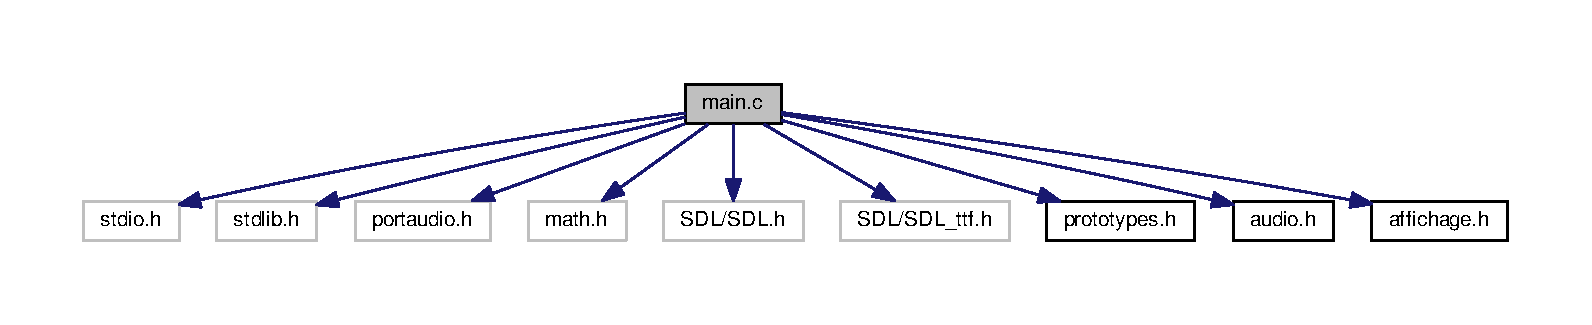
\includegraphics[width=350pt]{main_8c__incl}
\end{center}
\end{figure}
\subsection*{Fonctions}
\begin{DoxyCompactItemize}
\item 
\hyperlink{structBuffer}{Buffer} $\ast$ {\bfseries creer\+Buffer} ()\hypertarget{main_8c_aeac6a57809803dc95d2c2a55bde0611f}{}\label{main_8c_aeac6a57809803dc95d2c2a55bde0611f}

\item 
void {\bfseries push} (\hyperlink{structBuffer}{Buffer} $\ast$list\+Buffer, float $\ast$in)\hypertarget{main_8c_a30349e8abf179e11939304443da230fe}{}\label{main_8c_a30349e8abf179e11939304443da230fe}

\item 
void {\bfseries liberer\+Buffer} (\hyperlink{structBuffer}{Buffer} $\ast$list\+Buffer)\hypertarget{main_8c_a6934d2030dc10fb92693b66ad5f4891f}{}\label{main_8c_a6934d2030dc10fb92693b66ad5f4891f}

\item 
\hyperlink{structData}{Data} {\bfseries init\+Data} ()\hypertarget{main_8c_a55559823eed9a8f3c87934a44b1d766d}{}\label{main_8c_a55559823eed9a8f3c87934a44b1d766d}

\item 
int {\bfseries main} ()\hypertarget{main_8c_ae66f6b31b5ad750f1fe042a706a4e3d4}{}\label{main_8c_ae66f6b31b5ad750f1fe042a706a4e3d4}

\end{DoxyCompactItemize}


\subsection{Description détaillée}
Projet effet audio -\/ Fichier principal. 

L\textquotesingle{}objectif est de reproduire les effets audios souvent utilisés dans la musique. \begin{DoxyAuthor}{Auteur}
David B\+A\+L\+D\+A\+S\+S\+IN 

Sylvain B\+O\+U\+R\+G\+EA 
\end{DoxyAuthor}

%--- End generated contents ---

% Index
\backmatter
\newpage
\phantomsection
\clearemptydoublepage
\addcontentsline{toc}{chapter}{Index}
\printindex

\end{document}
